\documentclass[12pt]{article}
\usepackage[utf8]{inputenc}
\usepackage{float}
\usepackage{amsmath}


\usepackage[hmargin=3cm,vmargin=6.0cm]{geometry}
%\topmargin=0cm
\topmargin=-2cm
\addtolength{\textheight}{6.5cm}
\addtolength{\textwidth}{2.0cm}
%\setlength{\leftmargin}{-5cm}
\setlength{\oddsidemargin}{0.0cm}
\setlength{\evensidemargin}{0.0cm}

%misc libraries goes here
\usepackage{tikz}
\usetikzlibrary{automata,positioning}

\begin{document}

\section*{Student Information } 
%Write your full name and id number between the colon and newline
%Put one empty space character after colon and before newline
Full Name : Hakan Bostan \\
Id Number : 2098812 \\

% Write your answers below the section tags
\section*{Answer 1}

\subsection*{a.}
$a(a+c)^*b(a+c)^*b(a+c)^*cc$
\subsection*{b.}
$((b+c)(b+c))^*(((b+c)a)+(a(b+c)))((b+c)(b+c))^*$
\subsection*{c.}
$a^*bb^*aa^*bb^*aa^*b*$



\section*{Answer 2}

\subsection*{a.}
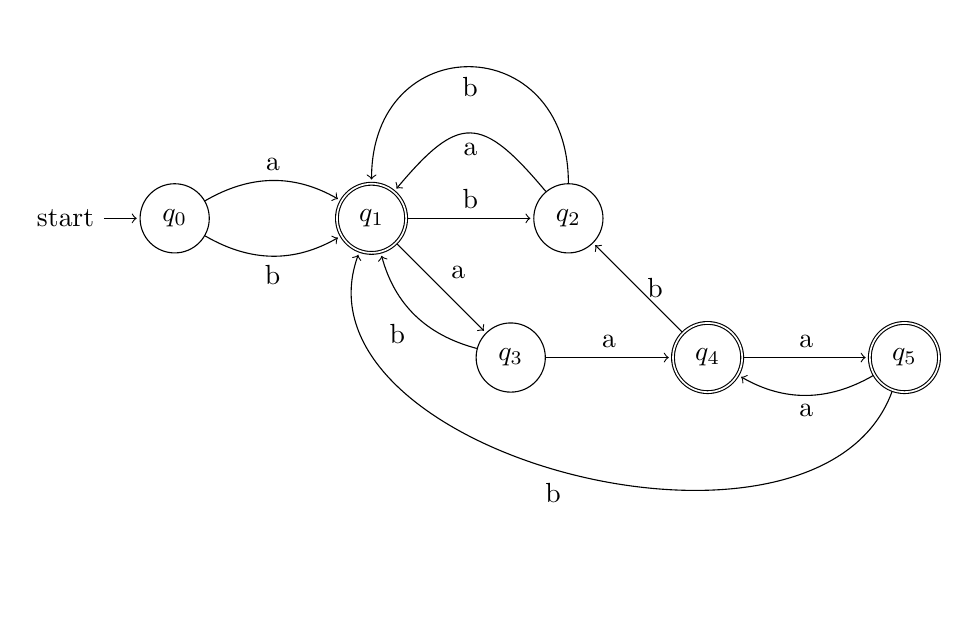
\begin{tikzpicture}[shorten >=1pt,node distance=2.5cm,on grid, auto]
	\node[state,initial] (q_0) {$q_0$};
	\node[state,accepting] (q_1) [right = of q_0] {$q_1$};
	\node[state] (q_2) [right = of q_1] {$q_2$};
	\node[state] (q_3) [below right = of q_1] {$q_3$};
	\node[state,accepting] (q_4) [right = of q_3] {$q_4$};
	\node[state,accepting] (q_5) [right = of q_4] {$q_5$};
	 \path[->]
	 (q_0) edge [bend left] node  {a} (q_1)
	       edge [bend right] node [swap] {b} (q_1)
	 (q_1) edge node {b} (q_2)
	       edge node {a} (q_3)
	 (q_2) edge [out=130, in=50,looseness=1.7] node  {a} (q_1)
	 	   edge [out=90, in=90,looseness=2] node {b} (q_1)
	 (q_3) edge node {a} (q_4)
	 	   edge [bend left] node {b} (q_1)
	 (q_4) edge node {a} (q_5)
	 	   edge node [right] {b} (q_2)
	 (q_5) edge [bend left] node {a} (q_4)
	 	   edge [out=250, in=250] node {b} (q_1);
\end{tikzpicture}
\subsection*{b.}
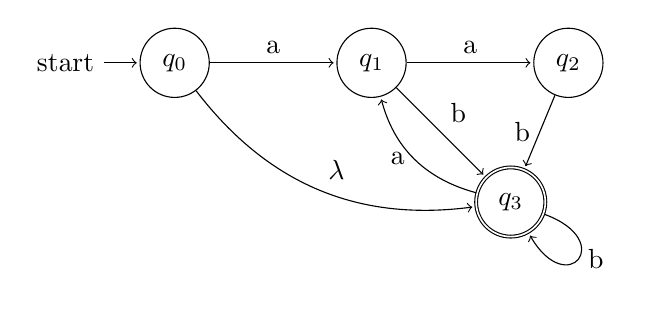
\begin{tikzpicture}[shorten >=1pt,node distance=2.5cm,on grid, auto]
	\node[state,initial] (q_0) {$q_0$};
	\node[state] (q_1) [right = of q_0]{$q_1$};
	\node[state] (q_2) [right = of q_1] {$q_2$};
	\node[state,accepting] (q_3) [below right = of q_1] {$q_3$};
	 \path[->]
	 (q_0) edge node  {a} (q_1)
	 	   edge [bend right] node {$\lambda$} (q_3)
	 (q_1) edge node {a} (q_2)
	       edge node {b} (q_3)
	 (q_2) edge node [left] {b} (q_3)
	 (q_3) edge [bend left] node [left] {a} (q_1)
	 	   edge [out=340,in=300,looseness=8] node [right] {b} (q_3);

\end{tikzpicture}
\section*{Answer 3}
\hspace{1.2cm}Family of regular languages are not necessarly closed under infinite unions. Take the set of languages $L_a=\lbrace 0^b1^a\rbrace$ over $\sum =\lbrace 0,1\rbrace$ (i.e. $L_1=\lbrace 01\rbrace$, $L_2=\lbrace 0011\rbrace$, ...).
The infinite union of these languages gives us $L=\lbrace 0^i1^i|i\in N\rbrace$. We will prove this language is not a regular language using Pumping Lemma.\\
\\
1. Assume that $L=\lbrace 0^i1^i|i\in N\rbrace$ is a regular language.\\
2. Let $m$ be the number from pumping lemma and let $s=0^m1^m$.\\
3. Since $s\in L$ and $|s|\geq m$ Pumping Lemma must apply.\\
Specifically $s=xyz$ where $|y|\neq 0$ and $|xy|\leq m$\\
$y=0^k$, $0<k\leq m$\hspace{1.3cm} $x=0^n$, $0<n<m$ \\$z=0^{m-k-n}1^m$\hspace{2cm} $s=0^n0^k0^{m-k-n}1^m$ \\
According to Pumping Lemma $xy^*z \in L$ must be true. Lets take $xyyz$.\\
$xyyz=0^n0^k0^k0^{m-k-n}1^m = 0^{m+k}1^m$.\\
Since $m+k\neq m$ it is clear that $xyyz\notin L$. We have a contradiction therefore $L=\lbrace 0^i1^i|i\in N\rbrace$ is not a regular language.\\

Overall the infinite union of regular languages does not necessarly make a regular language.
\section*{Answer 4}

1. Assume that $L=\lbrace a^ib^jc^{2j}|i\geq 0,j\geq 0\rbrace$ is a regular language.\\
2. Let $m$ be the number from pumping lemma and let $s=a^ib^mc^{2m}$.\\
3. Since $s\in L$ and $|s|\geq m$ Pumping Lemma must apply.\\
Specifically $s=xyz$ where $|y|\neq 0$ and $|xy|\leq m$\\
$y=b^n$, $0<n\leq m$\hspace{0.7cm}$x=a^rb^{m-n-r}$, $0<r<m$ \\$z=b^{r}c^{2m}$ \hspace{2cm} $s=a^rb^{m-n-r}b^nb^{r}c^{2m}$\\
According to Pumping Lemma $xy^*z \in L$ must be true. Lets take $xyyz$.\\
$xyyz=a^rb^{m-n-r}b^nb^nb^{r}c^{2m} = a^ib^{m+n}c^{2m}$.\\
Since $m+n\neq m$ it is clear that $xyyz\notin L$. We have a contradiction therefore $L=\lbrace a^ib^jc^{2j}|i\geq 0,j\geq 0\rbrace$ is not a regular language.

\section*{Answer 5}
Consider $L_{a}$ be a regular langugage which can be shown with a DFA $M =(Q,\sum ,\sigma ,q_0 ,F )$ . The complement of the $L_{a}$ is $\overline{L_a}$. 
$\overline{L_a}$ is accepted by the DFA $M' =(Q,\sum ,\sigma ,q_0 ,Q-F )$. And since we can show $\overline{L_a}$ with a DFA $\overline{L_a}$ is also a regular language.\\
\\
Also let $M_1=(Q_1,\sum_1 , \sigma_1 ,q_1,F_1)$ and $M_2=(Q_2,\sum_2 , \sigma_2 ,q_2,F_2)$ be the DFAs accepting the languages $L_a$ and $L_b$ respectively. We can construct
a new DFA in a way that it will accept an input only when both $M_1$ and $M_2$ accepts that input. That DFA can be shown as:
$$M'=(Q,\sum ,\sigma , q_0, F)$$ 
where\\
$Q=(Q_1 x Q_2)$ \\
$q=\langle q_1,q_2 \rangle$\\
$\sigma (\langle p_1,p_2 \rangle ,a)=(\sigma_1 (p_1,a), \sigma_2 (p_2,a))$\\
$F=(F_1 x F_2)$\\
Since we can construct this DFA $L_1 \cap L_2$ is also regular.\\
\\
We can write $L_1-L_2 = L_1 \cap \overline{L_2}$. In this expression, considering the above statements, if $L_2$ is regular then $\overline{L_2}$ is also regular.
And if $\overline{L_2}$ and $L_1$ is regular then $L_1 \cap \overline{L_2}$ is regular. Thus $L_1 - L_2$ is regular if both $L_1$ and $L_2$ is regular.

\section*{Answer 6}

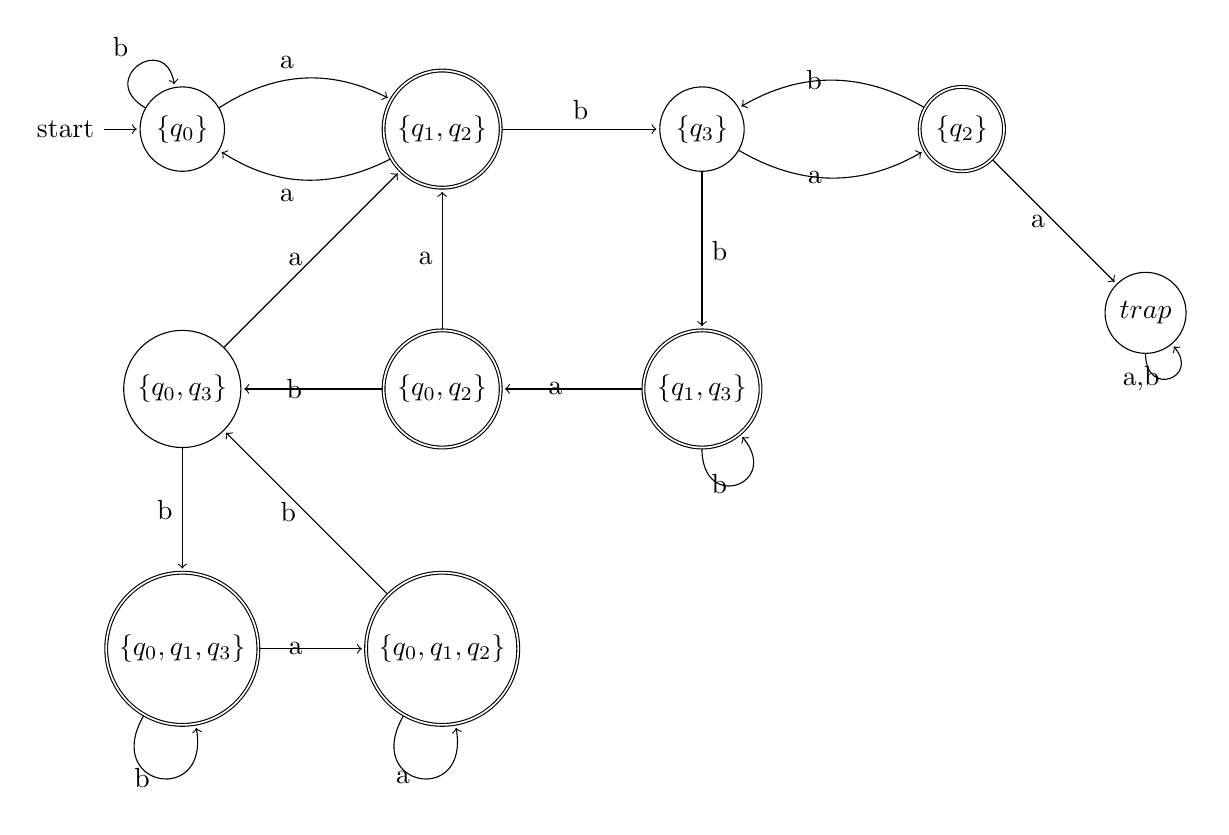
\begin{tikzpicture}[shorten >=1pt,node distance=3.3cm,on grid, auto]
	\node[state,initial] (q_0) {$\lbrace q_0\rbrace$};
	\node[state,accepting] (q_1) [right = of q_0] {$\lbrace q_1,q_2\rbrace$};
	\node[state] (q_2) [right = of q_1] {$\lbrace q_3\rbrace$};
	\node[state,accepting] (q_3) [right = of q_2] {$\lbrace q_2\rbrace$};
	\node[state] (q_4) [below right= of q_3] {$trap$};
	\node[state,accepting] (q_5) [below = of q_2] {$\lbrace q_1,q_3\rbrace$};
	\node[state,accepting] (q_6) [left = of q_5] {$\lbrace q_0,q_2\rbrace$};
	\node[state] (q_7) [left = of q_6] {$\lbrace q_0,q_3\rbrace$};
	\node[state,accepting] (q_8) [below = of q_7] {$\lbrace q_0,q_1,q_3\rbrace$};
	\node[state,accepting] (q_9) [right = of q_8] {$\lbrace q_0,q_1,q_2\rbrace$};
	\path[->]
	 (q_0) edge [bend left] node  {a} (q_1)
	 	   edge [out=150,in=100,looseness=4]node {b} (q_0)
	 (q_1) edge [bend left] node {a} (q_0)
	       edge node {b} (q_2)
	 (q_2) edge [bend right] node [left] {a} (q_3)
	 	   edge node [right] {b} (q_5)
	 (q_3) edge node [left] {a} (q_4)
	 	   edge [bend right] node [left] {b} (q_2)
	 (q_4) edge [out=270,in=310,looseness=4] node [left] {a,b} (q_4)
	 (q_5) edge [out=270,in=310,looseness=4] node [left] {b} (q_5)
	 	   edge node [left] {a} (q_6)
	 (q_6) edge node [left] {a} (q_1)
	 	   edge node [left] {b} (q_7)
	 (q_7) edge node [left] {a} (q_1)
	 	   edge node [left] {b} (q_8)
	 (q_8) edge [out=240,in=280,looseness=4]node [left] {b} (q_8)
	 	   edge node [left] {a} (q_9)
	 (q_9) edge [out=240,in=280,looseness=4] node [left] {a} (q_9)
	 	   edge node [left] {b} (q_7);
\end{tikzpicture}
The nodes of the above FA is from the power set of the node set of the original NFA. And if a node includes an accepting state node on the NFA, it is also an accepting node on the above FA.\\
Also this FA is minimal. There are no unneccesary or equivalent nodes.

\end{document}

​

